\section{Implementation}

\subsection{Project Structure}

One of the tasks that we have completed in this phase is to complete the design
of an structural framework that allows easy and incremental development of the
benchmarks. This section briefly describes the design.


\begin{table}[h]\small
\centering
\begin{tabular}{ | l | c |}
    \hline 
    Language &  Line Count \\ \hline
    Java & 7549 \\ \hline
    RenderScript & 1000 \\ \hline
    JNI/C++ & 2048 \\ \hline
    OpenCL & 480 \\ \hline
\end{tabular}
\caption{RSBench project line count breakdown.}
\label{table:breakdown}
\end{table}

Figure \ref{fig:package_structure} depicts the overview of the framework by mean
of the Java package structure. Figure \ref{fig:class_diagram} provides a closer
view at the organization of the classes related to the VectorAdd benchmark.

At a high level, we split the development of the graphical user interface (GUI),
from the development of each of the benchmarks, under the \fix{GUI} package and the
\fix{parboil} package in Figure \ref{fig:package_structure}, respectively. At this
stage, the GUI is simply to allow users to start running the benchmarks, and to 
display the status at the end of each benchmark, e.g., whether the benchmark has executed
successfully or failed. In the future, more features will be added, such as
display the progress of running the benchmarks, and the final scores of the
device. But we do not think that should be the focus of our development at this
moment.

The \fix{parboil} Java package is the core of the project. In this package, we also
identified the common functions, such as timing- and logging-related functions,
that are used across all the benchmarks. Those functions are further grouped in
classes, e.g., \fix{Timer} and \fix{Logger}, and implemented in the \fix{utils}
package. Each benchmark, e,g., \fix{bfs} or \fix{cutcp}, is implemented in a
separate package under the \fix{benchmark} package. Figure
\ref{fig:class_diagram} depicts the class diagram of the VectorAdd benchmark.
Other benchmarks have the same class structure. In order to implement a
benchmark, we just need to inherit for the \fix{ParboiBenchmark} class, which
layouts a common skeleton. For each benchmark, we have to implement a class to
read the input, for example \fix{VectorAddFileReader} class in this case. Each
computation kernel, e.g., for Java, threaded Java, RenderScript, or OpenCL, is
implemented in a separate class, e.g., \fix{VectorAddJava},
\fix{VectorAddThreadedJava}, \fix{VectorAddRS}, or \fix{VectorAddOpenCL},
respectively. These class inherits from the parent class of the benchmark, which
is the \fix{VectorAddBenchmark} in this case. This hierarchical design maximize
the code reuse between benchmarks, and between computation kernel.
It also allows for a consistent interface to run the benchmarks.

\subsection{Writing RenderScript kernels}
This section describes the general steps to write a computation kernel in
RenderScript for our benchmark.

By design, each RenderScript kernel executes to produce an \textit{element} of
the output. It is up to developers to define the granularity of an element. For
example, in the VectorAdd benchmark, an output element can be one, or two, or
three array elements of the output vector. This granularity essentially
determines the parallelism of the written RenderScript code. We often select the
finest granularity of the output element, e.g., one array element in this case,
to implement our RenderScript kernel.


In order to support this model, the RenderScript framework provides APIs to (i)
define the type of \fix{Element} for both input and output of RenderScript
kernels, and (ii) pack \fix{Element}s into \fix{Allocation}, which is the data
structure that is used to pass data back and forth between regular Java code and
RenderScript code.

A significant effort of our work is to determine efficient ways to convert input
data from original structure to the \fix{Allocation} structure with appropriate
\fix{Element} type. This conversion is also reflected at runtime through the
\textit{setup} time category of RenderScript execution.

After data has been packed into \fix{Allocation} objects, we move to write
RenderScript code in C99 format. The code need to be placed in a specific file
with .rs extension and a proper header, so that the Android Development Tools
(ADT) can automatically generate a Java class for it. The auto-generated Java
class provides interfaces to invoke the RenderScript code from Java code.

\begin{figure}[t!]
\centering
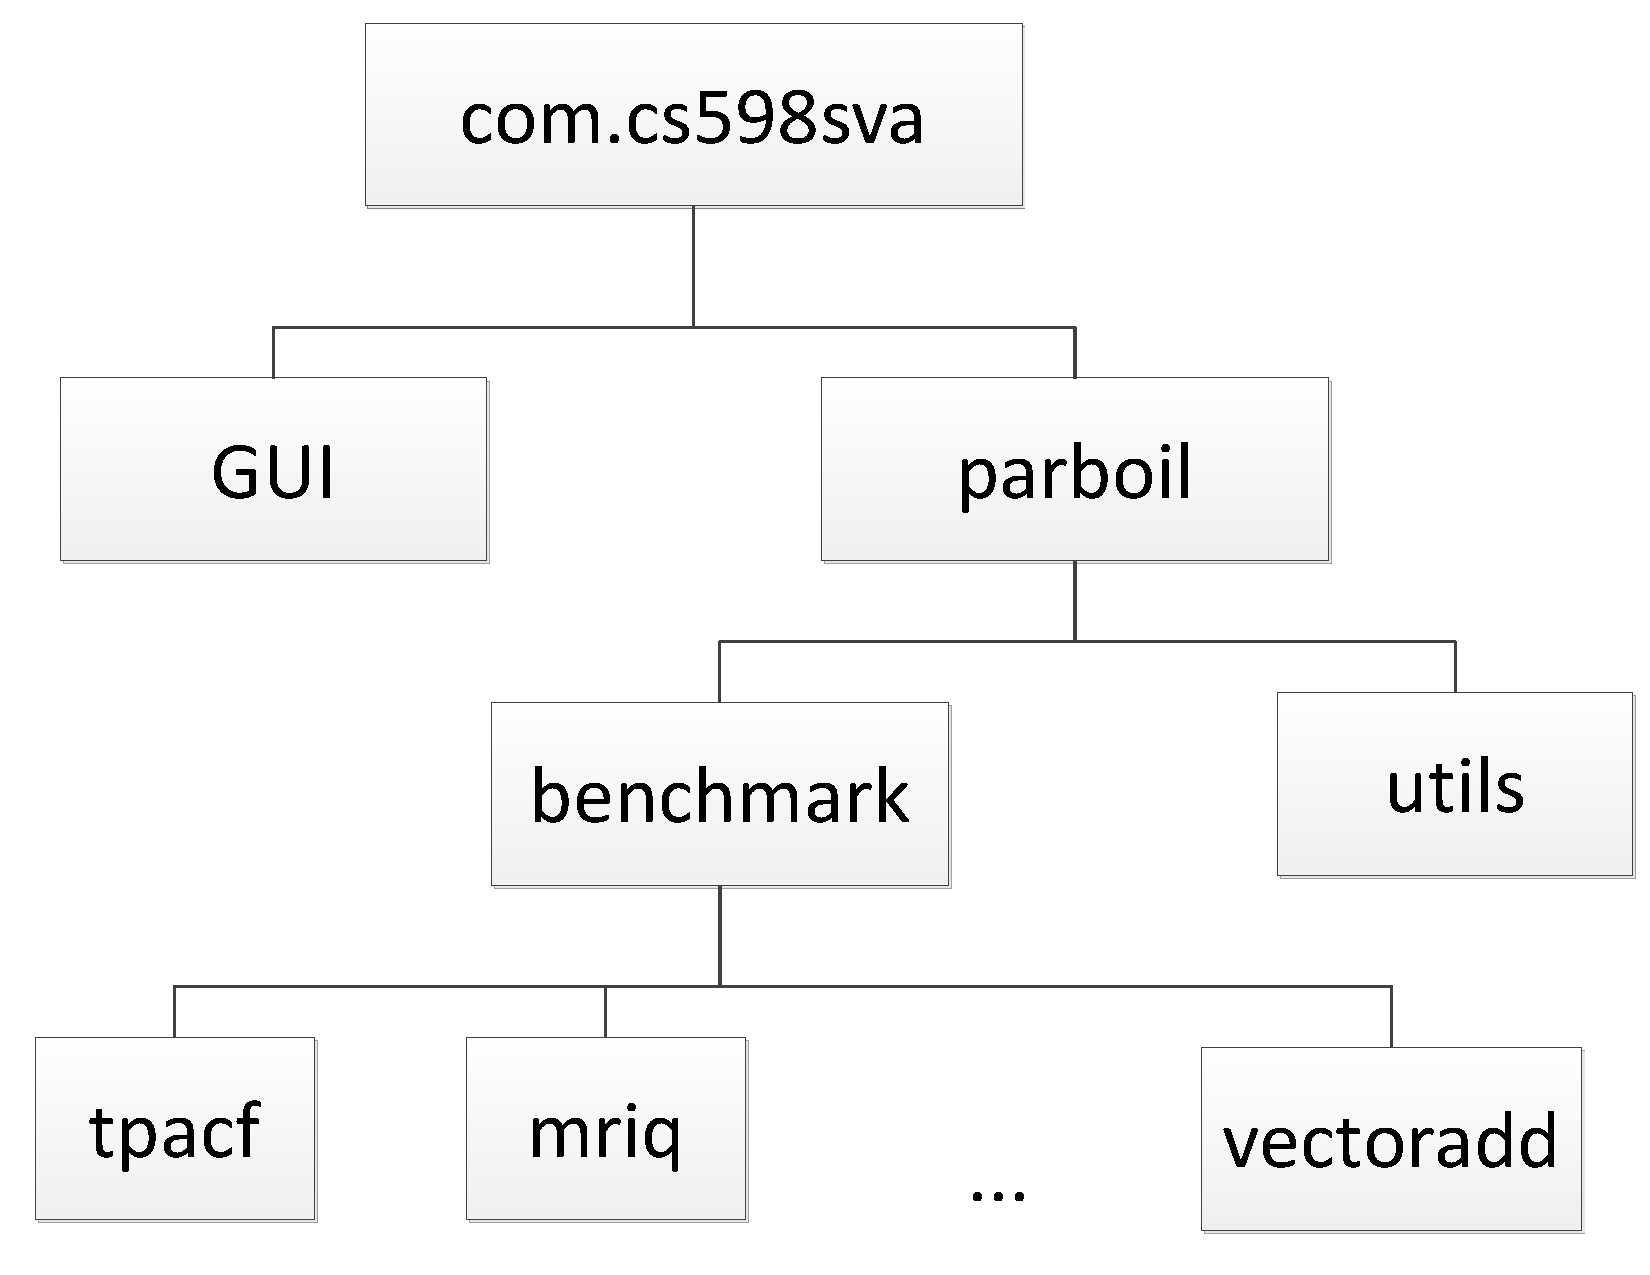
\includegraphics[scale=0.65]{figs/package_diagram.pdf}
\caption{RSBench Java package structure.}
\label{fig:package_structure}
\centering
\end{figure}


\begin{figure}[t!]
\centering
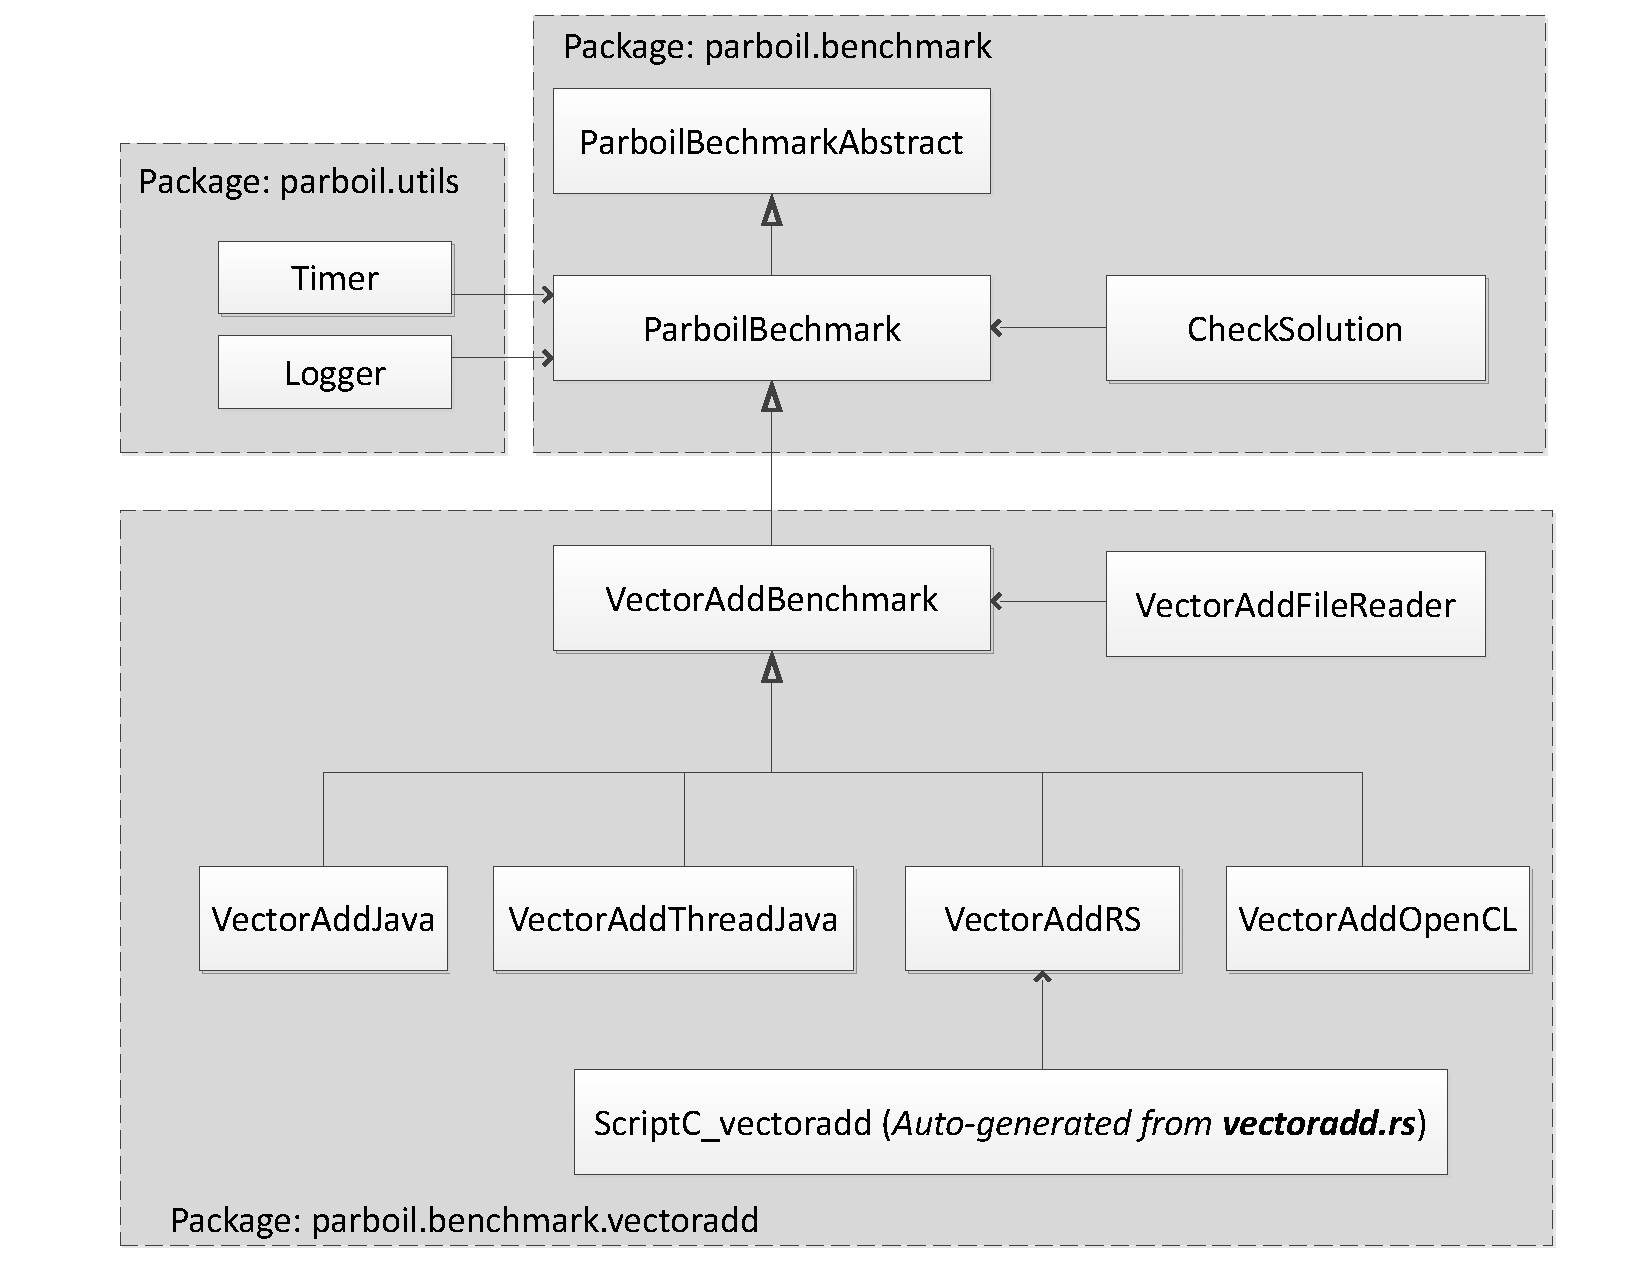
\includegraphics[scale=0.5]{figs/vectoradd_class_diagram.pdf}
\caption{Class diagram of the VectorAdd benchmark.}
\label{fig:class_diagram}
\centering
\end{figure}

\subsection{Timer}
The \fix{Timer} class is the most important utility in our benchmark. It
determines the accuracy and flexibility of our measurement. The \fix{Timer}
class utilizes Android's \fix{SystemClock}, which provides real-time clock at
nanosecond resolution. Each \fix{Timer} object consists of a flexible amount of
\fix{TimerElement} objects. Each \fix{TimerElement} object is a measure of a
particular execution segment, e.g., allocation time, setup time, and compute
time. In order to create a new \fix{TimerElement}, we just need to invoke the
\fix{Timer.start(category, message)} method at the beginning of the execution
segment we wish to measure (here category is a user defined category such as
``Compute'' or ``Setup'', while message is a message that further refines the
category such as ``Allocating temporary datastructures''). At the end of the
execution segment, we need to invoke the \fix{Time.stop()} method. The
time-stamp and elapsed time will be automatically computed and recorded. The
\fix{Timer} class also has a function that dumps all the recorded
\fix{TimerElement} to a SQLite database or serialize it to JSON format for
conveniently storing the results in an easily parsable format.

If a benchmark is run multiple times, for example, we run the compute part of
the implementation 5 times in our currently analysis, then the timer has code to
aggregate the results -- giving you the average time across runs.  Currently, we
do not exercise that code and we leave the statistical analysis to the parser
and visualizer.

\subsection{Output to Database}


\begin{figure}[t!]
\begin{verbatim}
{
	string Type,
	string Hardware,
	string Benchmark,
	string Implementation,
	string Category,
	string Message,
	long StartTime,
	long EndTime,
	long ElapsedTime,
	string Data,
	string Date,
}
\end{verbatim}
\caption{Database Columns.}
\label{fig:database}
\centering
\end{figure}

Unlike Parboil, which outputs the times to {\tt stdout}, we output our data into
a SQLite database (the schema is shown in table~\ref{fig:database}).  This affords us a few things.  First, since data is outputted
in the specified columns, we do not have to re-parse the output data.  Second,
timing information can be shared easily by copying the database.  Finally, we
can store more than just timing information -- for example we also store which machine the time has been taken on as well as which runtime is being used.

